\documentclass[]{auvsi_doc}
\setkeys{auvsi_doc.cls}{
	AUVSITitle={Unmanned Ground Vehicle Drop Subsystem Summary},
	AUVSILogoPath={./figs/logo.pdf},
}

% include extra packages, if needed

% Remove Heading Numbers
\setcounter{secnumdepth}{0}

% Remove Heading Numbers
\setcounter{secnumdepth}{0}


% include extra packages, if needed

\begin{document}

\begin{AUVSITitlePage}
\begin{artifacttable}
\entry{GV-005, 1.0, 10-30-2018, Wrote concept description, Kameron Eves, Andrew Torgesen}
\entry{GV-005, 1.1, 2-21-2019, Updated to reflect subsystem engineering, Jacob Willis, Brandon McBride}
\entry{GV-005, 1.2, 3-01-2019, Added performance summary and remaining development, Jacob Willis, Derek Knowles}
% additional \entry{} commands for extra rows in the revision table, if needed
\end{artifacttable}
\end{AUVSITitlePage}

% document contents (see below for LaTex commands that make your life easier)
\section{Introduction}
This document gives a more detailed description of the selected concept for the UGV delivery system. The concept selected during concept development was a parachute with fins. After considering the added complexity of fins, and the small benefit they provide, we determined to simply use a parachute.

\section{Description}

The UGV is to be loaded within the aircraft.
Upon a command from the flight controller system, a small hatch opens and the UGV falls out. 
The UGV is carried to the ground by a lightweight 36 inch nylon parachute, purchased from FruityChutes. 
The parachute is loaded onto the aircraft in a tube that allows the UGV to pull it out of the aircraft as it falls. This helps stop the tangling that can come from a folded parachute. To also prevent tangling, and to make for a more predictable drop, the parachute is folding according to GV-007. After exiting the aircraft the parachute will be opened by drag. This will slow down the system enough to allow the UGV to survive impact without damage. A visual depiction of our chosen system can be seen in Fig.~\ref{fig:side}.

\begin{figure}[h]
\centering
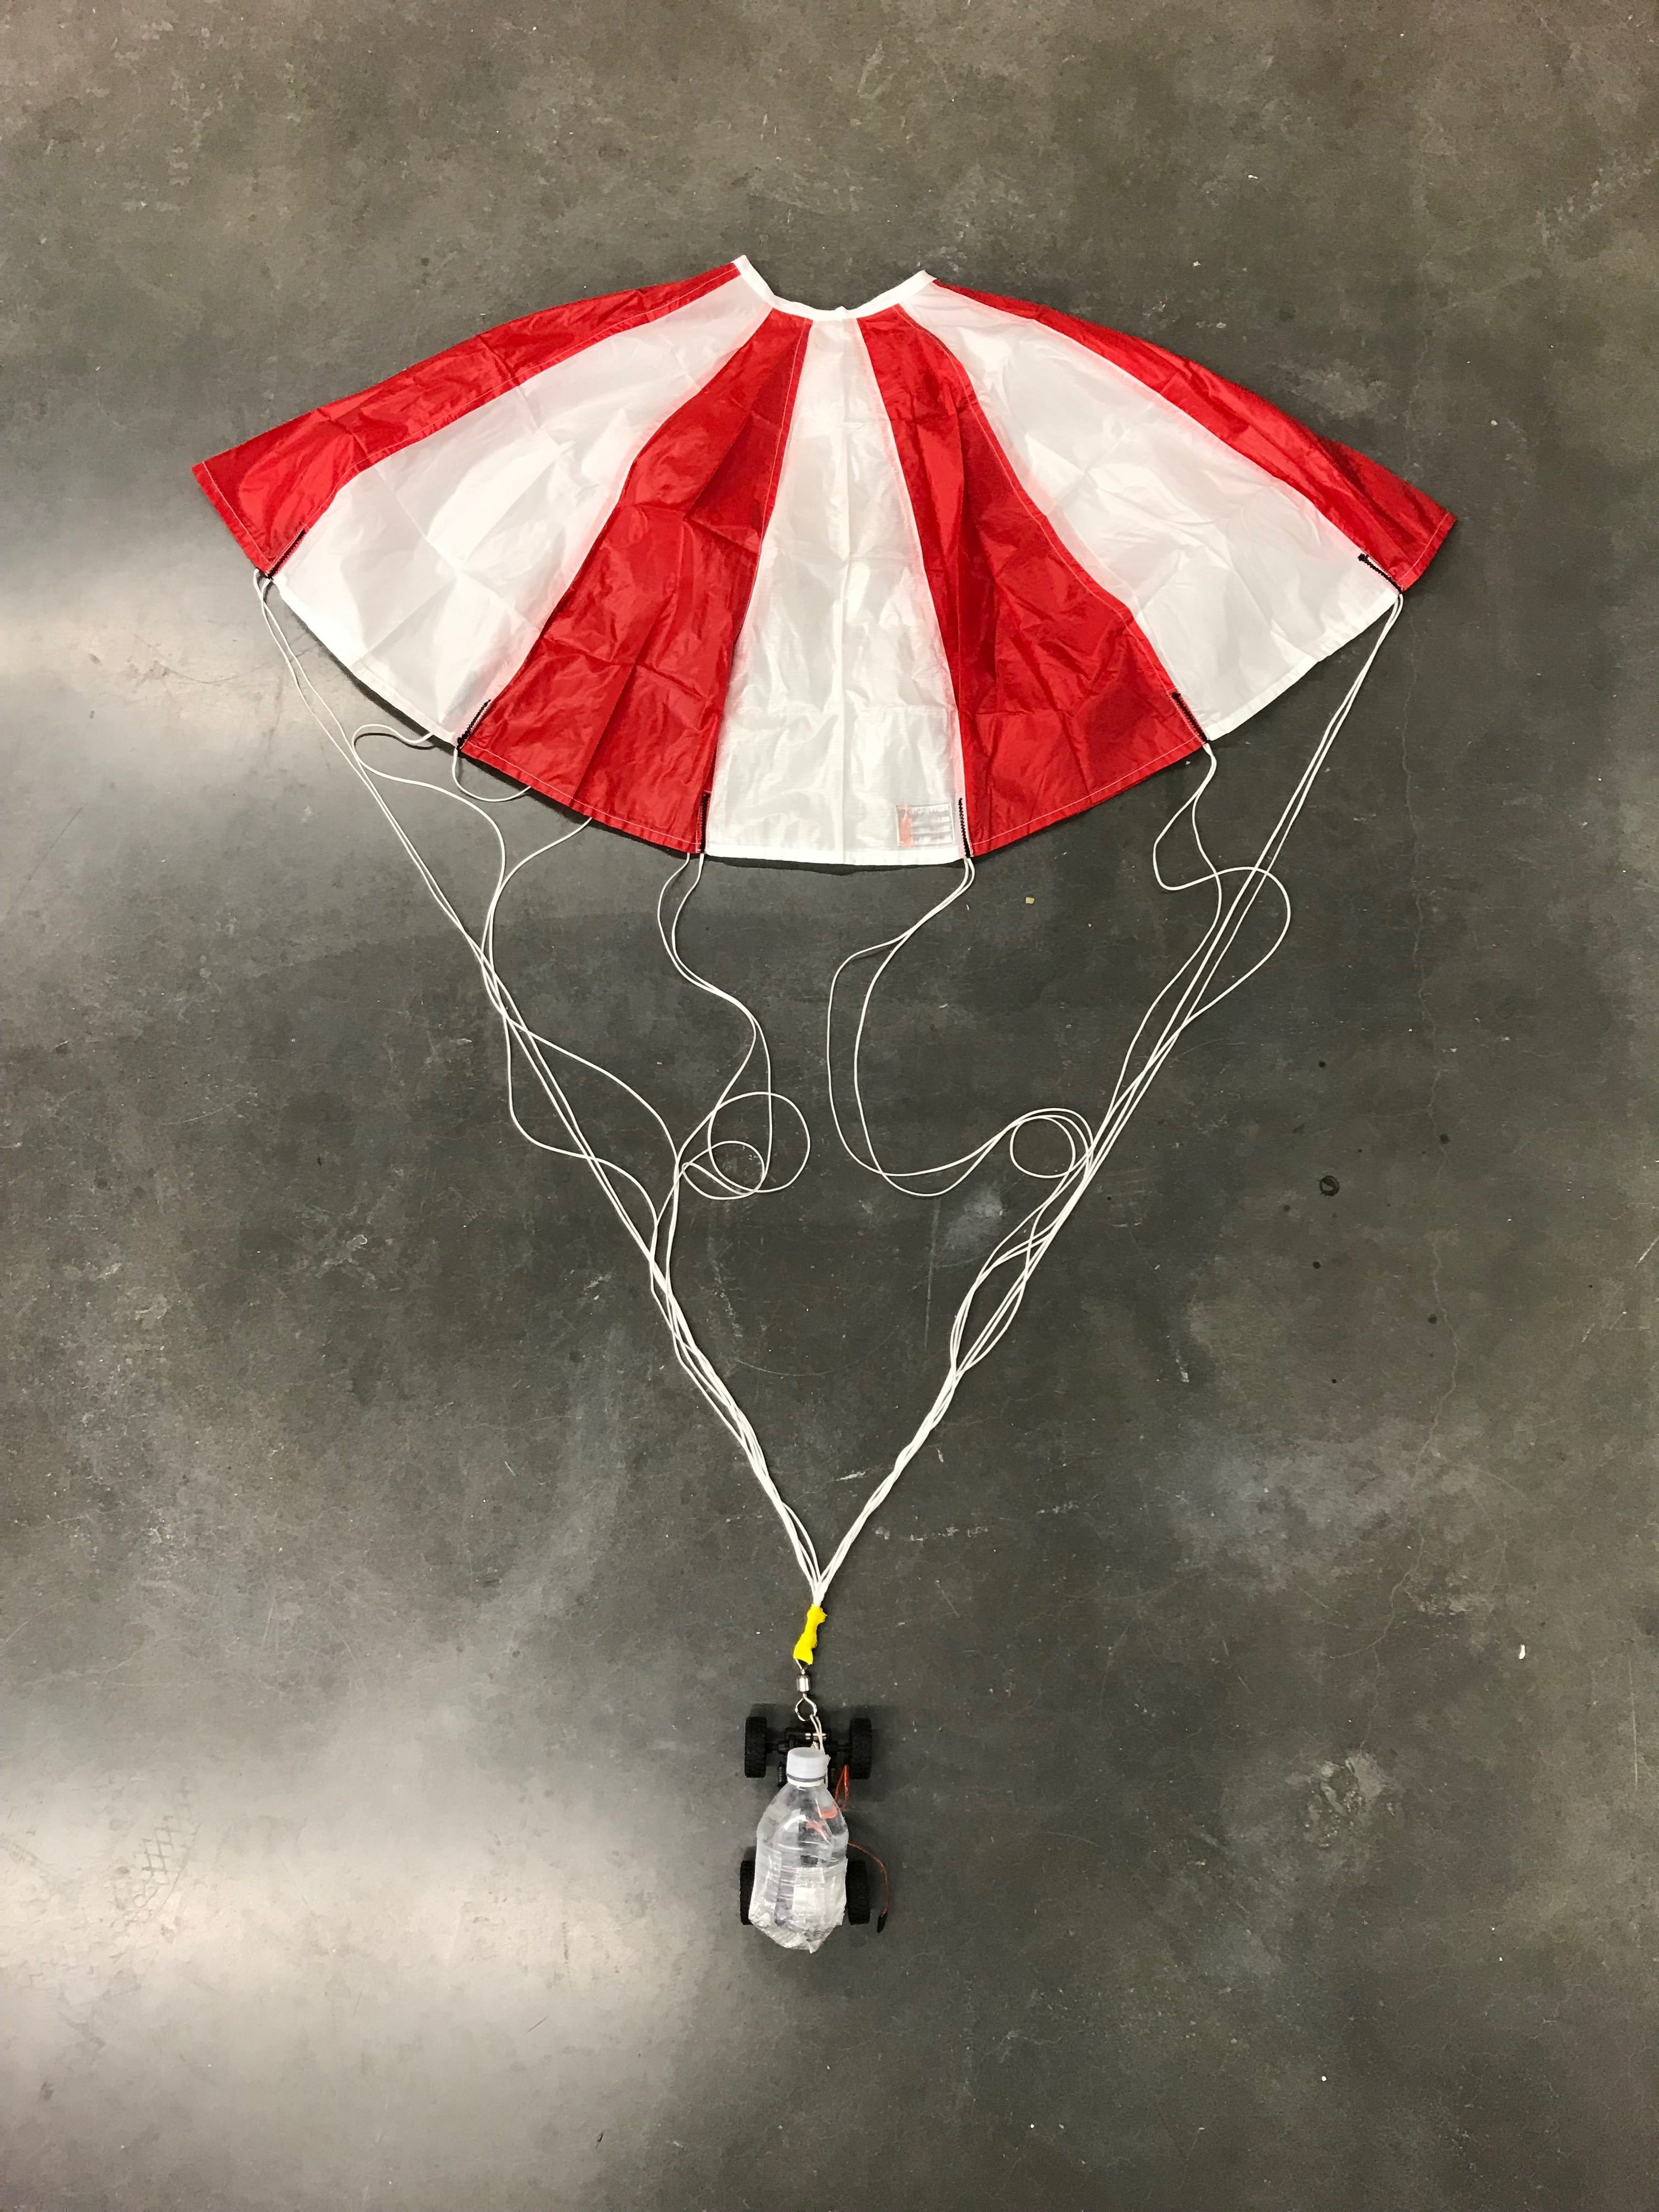
\includegraphics[width=90mm]{./figs/Parachute_Side.jpg}
\caption{Our parachute and simulated UGV as seen from the side.}
\label{fig:side}
\end{figure}

An accurate landing is an important part of the competition, and is the key success measure governing the design of the UGV drop system.
A hole in the top of the parachute improves the horizontal accuracy of the system by allowing a faster drop, but with more consistent aerodynamic effects.
This hole is known in the industry as a spill hole because it allows the air to spill out of the center of the parachute. 
 While this will not be enough to correct for large errors, it should be enough to ensure the system doesn't drift  too randomly. 
 
 The algorithm for dropping objects from a UGV, as detailed in \textit{Small Unmanned Aircraft: Theory and Practice} by Randy Beard and Tim McLain, is used to estimate the proper location to drop the UGV from in order to hit the target. This algorithm uses the wind and velocity of the aircraft to predict the best location to release the payload. A simulation of the drop, based on this algorithm is in GV-008. 
 The parachute adds some complexity to the algorithm, since the surface area and coefficient of drag are not constant during the drop. In order to more accurately predict the landing location of the UGV, the drop will be repeatedly timed, and the time will be used by the algorithm. This will allow us better accuracy in our drop algorithm than using a model of how the parachute drops. It also necessitates a highly repeatable deployment. These were design goals, and were focused on in the development of GV-006 and GV-007.

\section{Performance Summary}
The UGV subsystem performs within our defined acceptable range for all performance measures.
Due to its simple design, the mechanism weighs less and supports much more weight than expected. 
The parachute we selected is compact, yet allows a maximum landing velocity of three meters per second. This is sufficient to ensure a gentle landing of the UGV, meeting the competition requirements for the UGV drop. Because the full system must be integrated before testing drop accuracy, drop accuracy will be measured during system refinement.

\section{Remaining Development}
To complete the UGV drop subsystem we need to perform the following additional work. Due to dependencies on other subsystems, most of this development must be performed during system refinement.
\begin{enumerate}
	\item{Drop testing with the ground vehicle, rather than just a representative mass. This will allow us to check if the vehicle will remain on its wheels after landing.}
	\item{Timing the amount of time between the drop command and landing. This will allow us to best predict how the UGV will fall.}
	\item{Automatic drop location calculation given a target location. This relies on the autopilot to calculate an optimal drop location for hitting a given target.}
\end{enumerate}

\section{Conclusion}
Using the system described above, we are confidant in our ability to achieve a landing accuracy of within 25 feet. This is considered excellent performance in our key success measures and will give us 75\% of the points possible in this portion of the competition. 

\end{document}

